\documentclass[12pt]{article}

\usepackage[utf8]{inputenc}
\usepackage[T1]{fontenc}
\usepackage[ngerman]{babel}
\usepackage[ngerman=ngerman-x-latest]{hyphsubst}
\usepackage{csquotes}
\usepackage{hyphenat}
\usepackage{textcmds}
\usepackage{xspace}
\usepackage{listings}
\usepackage{amsmath}
\usepackage{amsfonts}
\usepackage{mathtools}

\usepackage{authblk}
\renewcommand*{\Authsep}{, }
\renewcommand*{\Authand}{ und }
\renewcommand*{\Authands}{ und }

\usepackage{geometry}
\geometry{a4paper, margin=1in}

\usepackage{graphicx}
\usepackage{chngpage}
\usepackage{calc}

\renewcommand{\lstlistingname}{Code}
\renewcommand{\lstlistlistingname}{Codeverzeichnis}

\usepackage{hyperref}
\hypersetup{
    colorlinks=true,
    linkcolor=black,
    filecolor=blue,
    urlcolor=blue,
    pdftitle={SLAB --- Labyrinth},
    pdfauthor={Nik Benson},
    pdfpagemode=FullScreen,
}
\urlstyle{same}

\usepackage{tikz}
\usepackage{pgfplots}
\usepackage{pgfplotstable}
\pgfplotsset{compat=1.18}
\usepgfplotslibrary{units}

\usepackage{booktabs}
\usepackage{siunitx}
\usepackage{csvsimple}


\usepackage{xcolor}
\definecolor{codegreen}{rgb}{0,0.6,0}
\definecolor{codegray}{rgb}{0.5,0.5,0.5}
\definecolor{codepurple}{rgb}{0.58,0,0.82}
\definecolor{backcolour}{rgb}{0.95,0.95,0.92}

\lstdefinestyle{java}{
    backgroundcolor=\color{backcolour},
    commentstyle=\color{codegreen},
    keywordstyle=\color{magenta},
    numberstyle=\tiny\color{codegray},
    stringstyle=\color{codepurple},
    basicstyle=\ttfamily\footnotesize,
    breakatwhitespace=false,
    breaklines=true,
    captionpos=b,
    keepspaces=true,
    numbers=left,
    numbersep=5pt,
    showspaces=false,
    showstringspaces=false,
    showtabs=false,
    tabsize=2
}

\lstset{style=java}

\DeclarePairedDelimiter\ceil{\lceil}{\rceil}
\DeclarePairedDelimiter\floor{\lfloor}{\rfloor}

\usepackage[backend=biber,style=iso-authoryear]{biblatex}
\bibliography{README}

\title{Semesterprojekt}
\author[1]{Nik Benson}
\affil[1]{\href{mailto:nik.benson@studmail.w-hs.de}{nik.benson@studmail.w-hs.de}}
\author[2]{David Borgert}
\affil[2]{\href{mailto:david.borgert@studmail.w-hs.de}{david.borgert@studmail.w-hs.de}}
\author[3]{Julian Frieling}
\affil[3]{\href{mailto:julian.frieling@studmail.w-hs.de}{julian.frieling@studmail.w-hs.de}}
\author[4]{Wilfried Ornowski}
\affil[4]{\href{mailto:wilfried.ornowkski@studmail.w-hs.de}{wilfried.ornowski@studmail.w-hs.de}}
\author[5]{Ulrich Steffen}
\affil[5]{\href{mailto:ulrich.steffen@studmail.w-hs.de}{ulrich.steffen@studmail.w-hs.de}}
\begin{document}
    \pagenumbering{gobble}
    \begin{titlepage}
    \maketitle
    \vspace{3cm}
    \begin{tabular}{l c r}
        
\includegraphics[width={0.45\textwidth}]{../assets/img/whs}
        & \hspace*{\fill} &
        \includesvg[width=0.45\textwidth]{../assets/img/netTrek}
    \end{tabular}
    \vspace*{\fill}
    \begin{flushleft}
        \Large{\textbf{Institution:} Westfälische Hochschule}\\
        \Large{\textbf{Modul:} \href{https://moodle.w-hs.de/course/view.php?id=36}{Student's Lab}} \\
        \Large{\textbf{Prüfer:} Prof. Dr. Martin Guddat}\\
        \Large{\textbf{Semester:} WiSe 22/23}
    \end{flushleft}
\end{titlepage}


    \pagenumbering{Roman}
    \setcounter{tocdepth}{3}
    \tableofcontents
    \addcontentsline{toc}{section}{Abbildungsverzeichnis}
    \listoffigures
    \addcontentsline{toc}{section}{Codeverzeichnis}
    \lstlistoflistings
    \newpage
    \pagenumbering{arabic}


    \section{Ziele}\label{sec:ziele}
        
\subsection{Vorwort}\label{subsec:Vorwort}

Seit 5000 Jahren\footnote{\url{https://www.math.stonybrook.edu/~tony/whatsnew/oct15/labyrinths.html}} fasziniert das Labyrinth, der Irrgarten bzw. Maze den Menschen. Dieser Faszination wir sind auch nachgegangen und untersuchten das Erstellen von Labyrinthen sowie die visuelle Darstellung. Auch haben wir Algorithmen zum Lösen von Labyrinthen untersucht. Unzählige Prototypen, meist mit p5js\footnote{\url{https://p5js.org}}(einer Portierung von Processing\footnote{\url{https://processing.org}}  mit Java nach Javascript)  wurden erstellt bzw.  vorhandene Quellen untersucht.

	Wir standen vor der Entscheidung Processing nativ zu verwenden, mit eingeschränkter Entwicklungsumgebung Processing Development Environment (PDE)\footnote{\url{https://processing.org/environment}},  oder zu versuchen Processing in Java\footnote{\url{https://happycoding.io/tutorials/java/processing-in-java}}, wie ein Framework, in einer gängigen Entwicklungsumgebung zu nutzen. Und haben uns für die Nutzung von Processing als Framework mit der beliebten Java IDE Intellj von jetbrain entschieden. So gestaltet sich die Entwicklung leichter und wir konnten Maven als buildtool und git zur Versionsverwaltung leicht einsetzen. Wir starteten mit einer alten Processing Version 3.5.4 weil sie als einzige im Maven Repository zu finden war. 

	Dieses unterstütze 3D open GL nicht korrekt auf mac os mit Apple silicon. Später konnten wir auf eine aktuelle Processing Version 4.1.1 wechseln. Auch diese war nicht perfekt gepackt im Maven Repository. Das haben wir in dann zu Fuß selber gemacht. Wir stießen auf fehlerhafte Einstellungen in IntelliJ für Maven Projekte in der mac os Version. Und konnten auch dieses lösen.

\subsection{MVP}\label{subsec:mvp}
	Unser MVP(Minimum-Viable-Product) für das Projekt "Labyrinth"  wurde nach ausführlichen Diskussionen während der ersten Sitzungen in Zusammenarbeit aller Anwesenden festgelegt. Es wurde entschieden das wir für ein minimales, sowie präsentierbares Produkt mindestens folgende Milestones erfüllen wollen.
	
	- Ein (rechteckiges)2d Labyrinth generieren
	
	- Eine Topdown Ansicht (für ein 3d Labyrinth)
		
	- Ein Lösungsalgorithmus
	
	- Eine Möglichkeit den Lösungsweg im Labyrinth anzeigen lassen
		
	Während der Arbeit am Projekt hat sich allerdings herausgestellt das der Fokus des Backend Teams vielmehr auf dem Generierungs- als auf dem Lösungsalgorithmus lag. Durch diese Verschiebung des Fokus, haben wir den Lösungsalgorithmus daher auch nicht im finalem Produkt integriert und unsere Milestones zur Wegfindung nicht erreicht.
	
	Wie genau sich die Erarbeitung zum implementierten Algorithmus gestaltet hat und eine genauere Beschreibung dessen findet sich im Abschnitt 3. / "Generieren eines rechteckigen Labyrinths" wieder.

    \subsubsection*{Labyrinth wird generiert mit Java}
		Nachdem wir die Minimum-Ziele definiert und ausformuliert haben mussten wir uns auch zwangsweise mit der Frage beschäftigen welche Tools wir zur Arbeit am Projekt benutzen wollen.
		
		Detaillierte Infos zu den verwendeten Tools befinden sich im Abschnitt 2. / "Tooling".
		
		Warum dieser Zusatz zu dem bereits definierten Milestone der Labyrinthgenerierung jedoch wichtig war ergibt sich aus unserer Entscheidung den Algorithmus Processing unabhängig zu bauen. Daraus folgte das wir eine Datenstruktur(Output) in Java generieren welche wir dann an Processing übergeben. Die Daten können dann innerhalb der Processing-Umgebung vom Frontend Team weiterverwendet werden und somit auch graphisch dargestellt werden.
		  
		Daraus ergab sich folgende, verbesserte Formulierung unseres zuvor gesetzten Milestones:    
		
		Ein (rechteckiges)2d Labyrinth in Processing darstellen -> welches zuvor in Java und unabhängig von Processing generiert wurde.
		
    \subsubsection*{Labyrinth wird in Topdown Ansicht dargestellt mit Processing}
    	Implementiert in dem Milestone der Topdown Ansicht befindet sich die Implementierung einer 3d Darstellung des Labyrinths. Diese Implementierung wurde vom Frontend Team basierend auf dem Code zur 2d Darstellung erarbeitet. Basierend auf der Möglichkeit das Labyrinth nun 3d Darstellen zu können, diente dieser Schritt als Grundlage um eine Sinnvolle Topdown Ansicht zu implementieren.
    	
    	Dementsprechend stellt dieser Milestone einen wichtigen Schritt in unsere Projektarbeit da, da dieser den Wechsel von 2- in 3d beinhaltet.


\subsection{Milestones}\label{subsec:milestones}
    Bereits zu beginn gab es neben den festgelegten minimalen Milestones für das MVP einen regen Austausch über mögliche Features(Milestones), welche wir gerne implementieren würden, realistisch gesehen den Rahmen der Projektarbeit aber überschreiten.
    
    Nichtsdestotrotz haben sich aus diesen Überlegungen einige interessante Milestones ergebe welche wir nach der Fertigstellung des MVP erarbeiten könnten.
    
    Eine Auflistung welche Features zur Diskussion standen und welche wir tatsächlich im Projekt noch integriert haben findet sich im folgendem Text.


    \subsubsection*{Bewegen durch das Labyrinth}
        Das Bewegen durch das Labyrinth war eines der wichtigsten Features in Bezug darauf unser Projekt als tatsächliches "Spiel" zu bezeichnen. Das Feature impliziert neben dem reinen bewegen durch, auch die Möglichkeit zum beenden des Labyrinthes und hat unser MVP von der reinen Darstellung um grundlegende Interaktionen mit dem Labyrinth erweitert.

    \subsubsection*{First Person}
        Basierend auf den zwei zuvor Vorgestellten Features ist die First Person Ansicht der letzte Milestone, welchen wir nach dem MVP noch implementiert haben. 
        
        Die First Person Ansicht basiert auf dem Feature der 3d Implementierung und würde ohne diese keine sinnvolle Implementierung zulassen. Das Feature der First Person Ansicht war dementsprechend ein wichtiges Feature im Bereich der 3d Darstellung und setzt eine klare Unterscheidung zwischen 3- und 2d Ansicht welche im Gegensatz zu Topdown Ansicht im 3d einen deutlich signifikanteren und insbesondere erkennbaren Unterschied macht.    

    \subsubsection*{Varianten bei der Generierung}
        Varianten bei der Generierung sollten der Grundstein für einen möglichen Level-Editor werden. Intern hätten verschiedene Generierungsalgorithmen für mehr Variation bei den Labyrinthen gesorgt während sie extern eine Basis für Endnutzer bei der Nutzung des Level-Editors hätten bieten können.
        
        Da das Backend Team allerdings durch die Implementierung eines eigenen Algorithmus für das MVP bereits viel Zeit benötigt hat, hat es dieses Feature nicht in das Endprodukt geschafft. 


    \subsubsection*{Level Editor}
        Der Level-Editor war eines unserer "advanced" Features und war die nächste Stufe der Generierungsvarianten. Dementsprechend sollte der Editor das erste große Feature sein mit welchem auch Endnutzer des Projekts eigene Level generieren und darstellen können. 
        
        Grundlage hierfür war das obige Feature bezüglich der Varianten (siehe "Varianten der Generierung" für Details) und genauso wie das vorherige Feature hat es auch der Editor nicht ins fertige Produkt geschafft. 


    \subsubsection*{P5JS}
		P5JS ist das Gegenstück zu Processig(Java), jedoch mit Javascript. So kann man ein Programm in P5JS im Web-Browser ausführen. So könnte unser Program auf einem Server laufen  und wäre Weltweit erreichbar. 
		
		Dieses Feature hat es aus zeitlichen Gründen nicht in unser Endprodukt geschafft.
		 

    \subsubsection*{Ball}
    	Eine Version unseres Programms für ein Android-Tablet / iPad. Bei dieser wäre es möglich einen Ball durch neigen des Tablets in eine Richtung zu rollen.
    	
    	Dieses Feature hat es nicht in das Endprodukt geschafft. 

		
 
		
  



    \section{Tooling}\label{sec:tooling}
        Auch die verwendeten Tools haben einen entscheidenden Einfluss auf unser Projekt gehabt.
Deshalb sind im Folgenden die wichtigsten 3 dargestellt.


\subsection{Git --- Versionskontrolle}\label{subsec:git-----versionskontrolle}
    Git ist ein Versionierungssystem, das textbasiert Änderungen erkennen und verwalten kann.
    Dies bietet insofern einen Vorteil in diesem Projekt gegenüber Alternativen, wie Bitbucket, die nicht auf Textebene arbeiten, dass Zeichenweise Änderungen erkannt und zusammengeführt werden können.
    Sofern Änderungen in verschiedenen Zeilen sind, meist sogar automatisch.


    Diese Änderungen sind dabei in Commits unterteilt.
    So können wir unbeirrt entwickeln, ohne uns Sorgen machen zu müssen, ob wir etwas Falsches löschen.


    Auch können wir so mit der Platform \href{https://github.com/WHS-SLAB-WiSe22-23-P1/Labyrinth}{GitHub} kollaborieren.
    Dies ist in den folgenden beiden Abschnitten~\ref{subsubsec:git--flow-----branching} und~\ref{subsubsec:conventional-commits} genauer dargestellt.

    \subsubsection{Git--Flow --- Branching}\label{subsubsec:git--flow-----branching}
        \begin{figure}
            \centering
            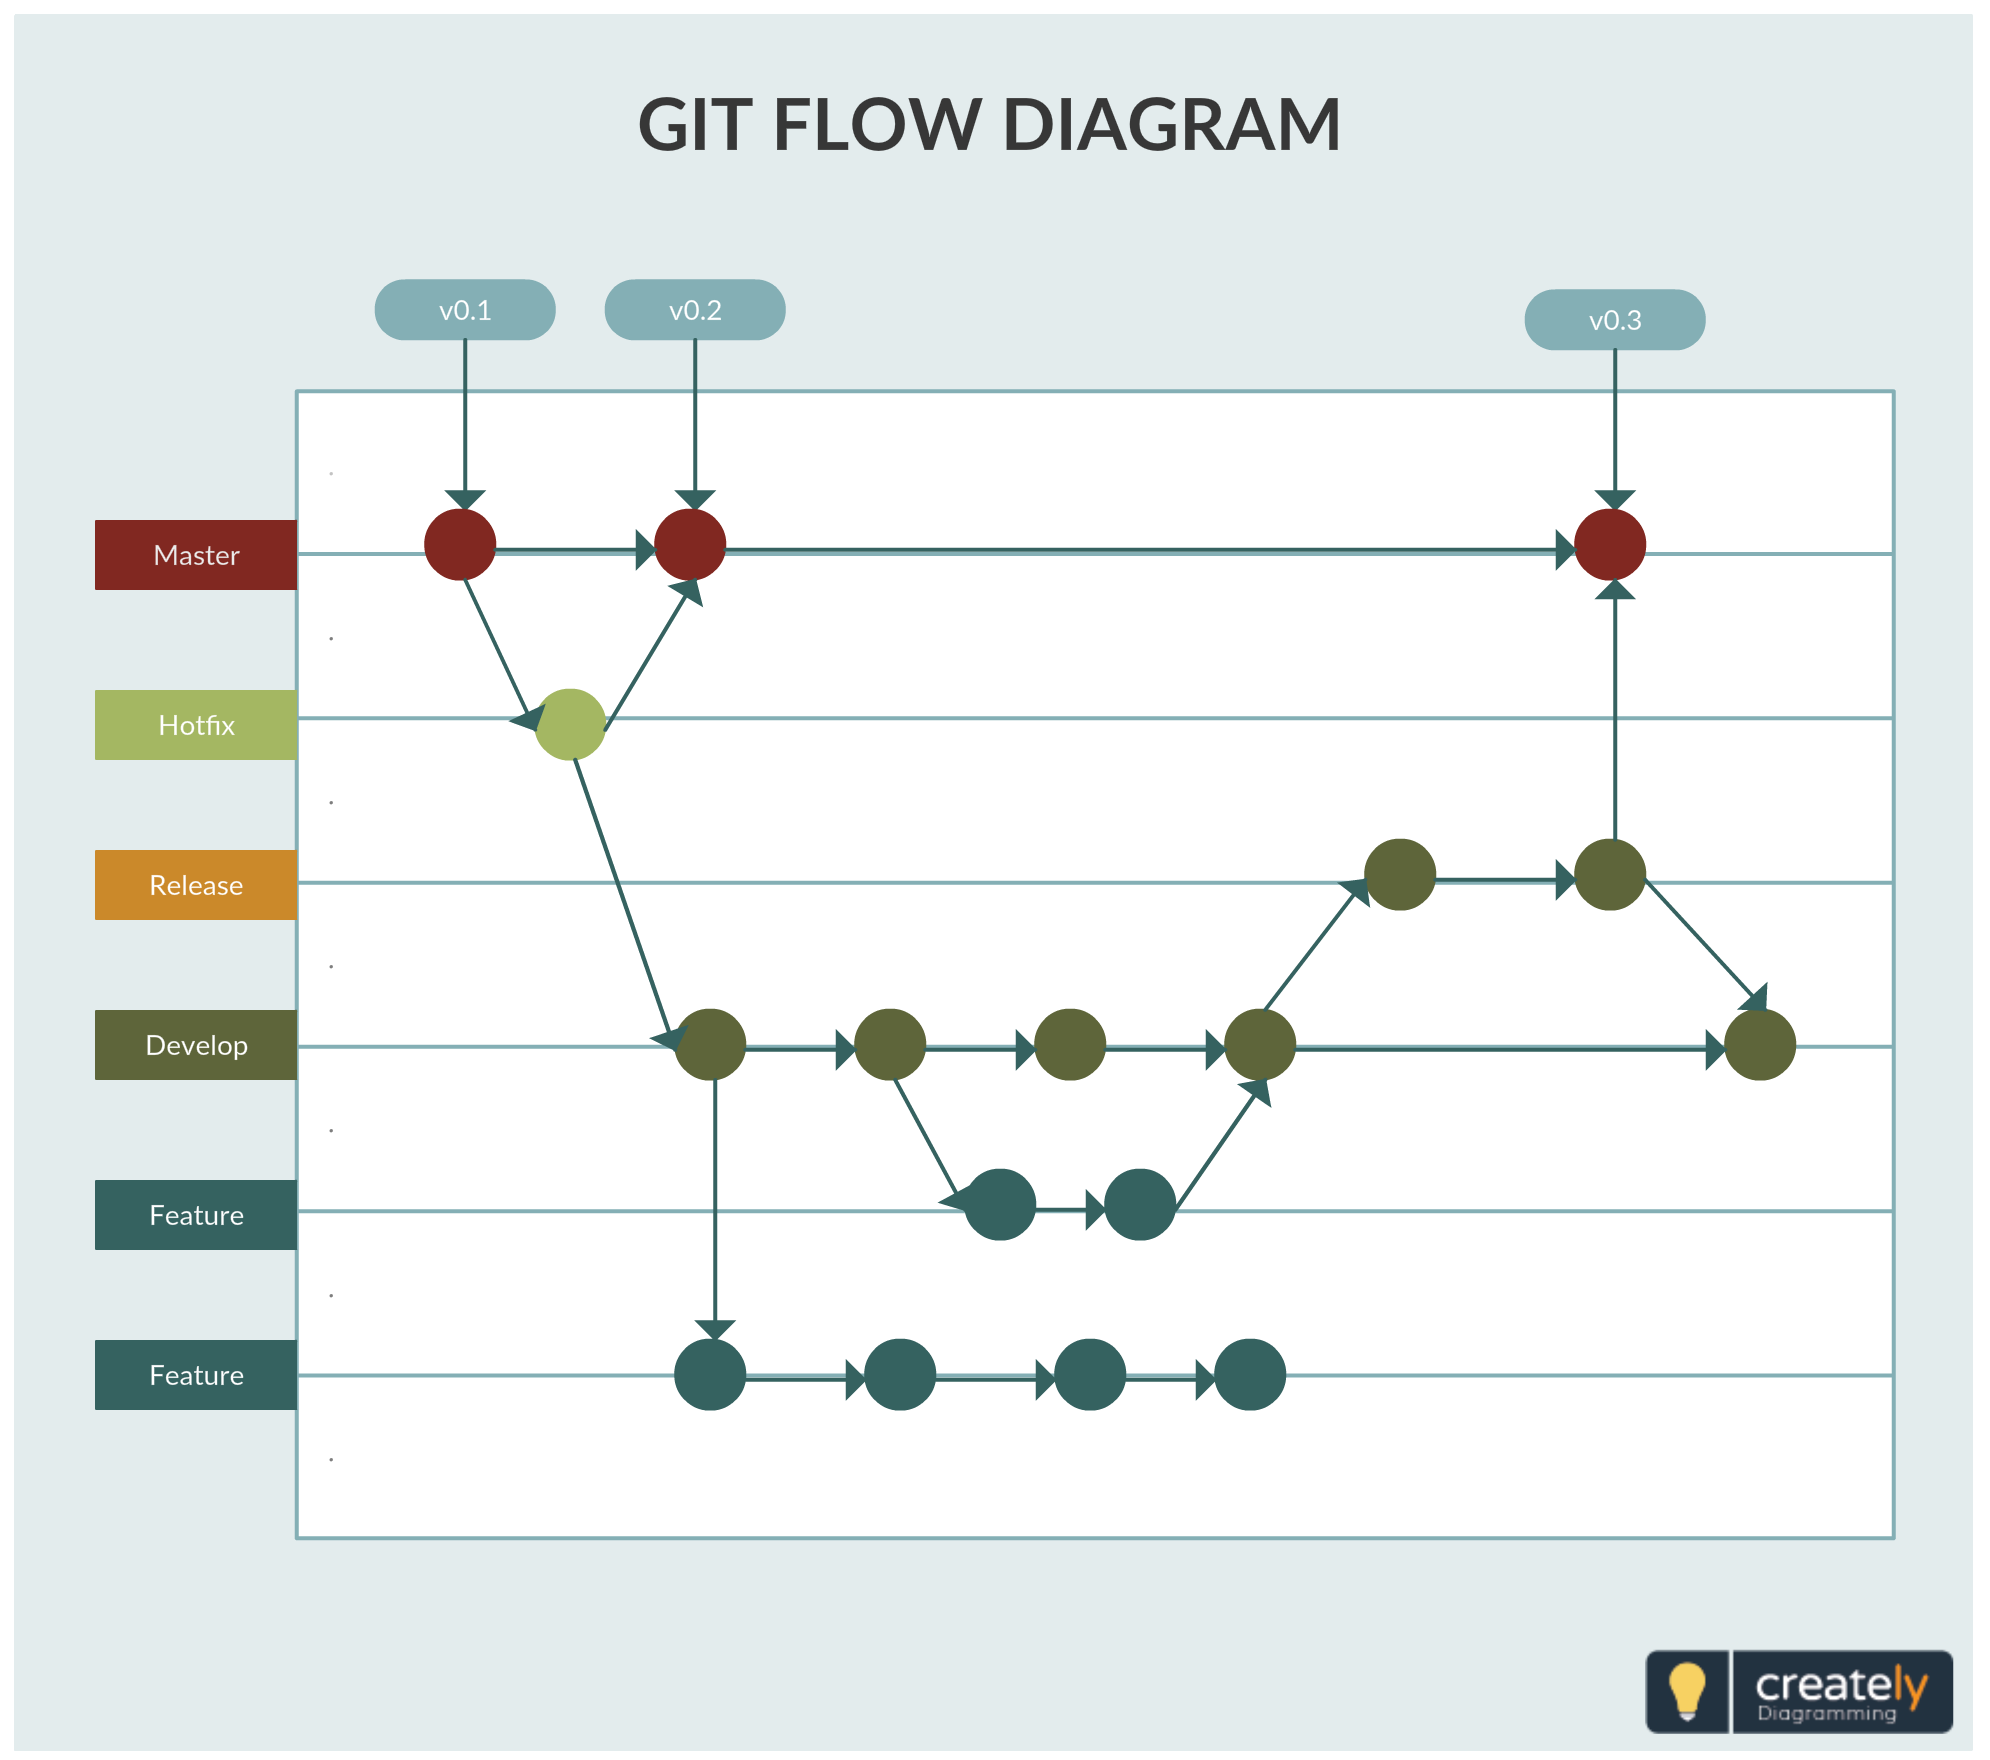
\includegraphics[width=\paperwidth-2in]{../assets/img/git_flow}
            \caption{Branches im Git--Flow Modell~\autocite{creately-no-date}}
            \label{fig:git-flow}
        \end{figure}
        Branching ist eines der wichtigsten Konzepte der Versionskontrolle.
        Es erlaubt mehreren Entwicklern gleichzeitig an verschiedenen Features zu arbeiten.
        Ein Branch ist dabei ein Pointer auf einen Commit.
        Werden zwei Branches zusammengeführt, so sprechen wir von einem Merge.
        Git-Flow ist ein Modell, wie Branches angelegt und strukturiert werden sowie was wohin gemerged wird.


        \paragraph{Main} (In Abbildung~\ref{fig:git-flow} Master genannt) beschreibt dabei die aktuelle Release--Version.
            Es wird niemals direkt in \textbf{Main} committed.


        \paragraph{Develop} ist die aktuelle Entwicklungs--Version.
            Hier wird getestet, ob \textbf{Features} gut zusammen funktionieren, also keine semantischen Fehler durch einen Merge aufgetreten sind.
            Es dürfen nur Commits erstellt werden, die einen solchen Fehler beheben.


        \paragraph{Features} sind nicht zwangsläufig neue Features.
            Es kann sich dabei auch um einen Bugfix oder Dokumentation, etc.\ handeln.
            In einem \textbf{Feature} arbeitet nur ein Entwickler zur selben Zeit.
            Features haben \textbf{Develop} als Upstream und werden nach fertigstellung in \textbf{Develop} gemerged.


        \paragraph{Hotfixes} sollen kritische Bugs schnell fixen.
            Es sind \textit{Shortcut Features}, die mit upstream \textbf{Main} direkt wieder in \textbf{Main} gemerged werden.
            Anschließend wird \textbf{Main} in \textbf{Develop} gemerged, damit alle wieder mit dem aktuellsten Stand arbeiten.


        \paragraph{Releases} haben \textbf{Develop} als Upstream und werden in \textbf{Main} gemerged.
            Sie sind für die Release--Vorbereitung gedacht.
            Hier wird zum Beispiel die Version angepasst oder mit Conventional Commits~\ref{subsubsec:conventional-commits} ein Changelog generiert.
            Nach dem Release wird \textbf{Main} in \textbf{Develop} gemerged.


        \paragraph Wir nutzen eine etwas abgespeckte Version ohne \textbf{Release}-- sowie \textbf{Hotfix}--Branches, da wir keine Releaseversion verwalten müssen.


    \subsubsection{Conventional Commits}\label{subsubsec:conventional-commits}
        Mit dieser, ursprünglich für das Web--Framework Angular entwickelten Konvention lassen sich git leserliche sowie leicht zu parsende Commit Nachrichten verfassen.
        Sie entsprechen dem Format \qq{<feat|fix|build|chore|ci|docs|style|refactor|perf|test>(<scope>): <message>}.


        Die Änderungen sind zunächst in eine der \textbf{Kategorien} zu unterteilen.
        Bei komplexen Projektspezifikationen können auch andere als die aufgeführten auf Projektebene spezifiziert werden.


        Anschließend kann ein \textbf{Scope} angegeben werden.
        Dies bietet sich vor allem bei einem Monorepo bzw.\ Multi--Module--Setup, wie unserem an.
        Unsere \textbf{Scopes} entsprechen dem bearbeiteten Maven~\ref{subsec:maven-----build--management} Modulen.
        Lässt sich kein eindeutiges \textbf{Scope} bestimmen, oder ist das Projekt zu klein, wird das \textbf{Scope} ausgelassen.


        Die \textbf{Nachricht} beschreibt, was geändert wurde.
        Sie sollte so formuliert werden, dass das thema der Änderung in wenigen Worten verständlich ist.


        Das Format muss nicht in Feature--Branches verwendet werden, wenn diese gesquashed (komprimiert) werden.
        Es sollte aber bei allen Commits, die in Develop landen angewendet werden.
        Daraus können dann sehr einfach Changelogs und ähnliches generiert werden.


\subsection{Maven --- Build--Management}\label{subsec:maven-----build--management}
    Mit Maven lässt sich der Aufbau des Projekts beschreiben.


    Zum einen müssen die Abhängigkeiten (Dependencies) lediglich als eine URI angegeben werden.
    So muss sich nicht jeder dieselben JARs herunterladen und in der IDE~\ref{subsec:intellij-----ide} manuell einbinden.


    Aber auch lässt sich die Software in Module unterteilen.
    So muss nicht alles in dieselbe JAR komprimiert werden und Front-- und Backend können im selben Repository arbeiten.
    Aber auch gemeinsame Abhängigkeiten, wie unser Datenmodell lassen sich damit erstellen.


    Alles in allem kümmert sich das Tool darum, dass alle nötigen Module in der richtigen Reihenfolge kompiliert und zusammengefügt werden.


    Ein großes Problem war es, dass die neuste major Version von Processing nicht mit Maven veröffentlicht wurde.
    Wir haben also ein Kompilat des öffentlichen Repositories eines Drittanbieters genutzt.
    Damit hatten wir allerdings lediglich die Core Library zur Verfügung.


\subsection{IntelliJ --- IDE}\label{subsec:intellij-----ide}
    Mittels Maven~\ref{subsec:maven-----build--management} war eis ein leichtes, Processing in dieser \textit{\textbf{I}ntegrated \textbf{D}evelopment \textbf{E}nvironment} einzubinden.
    Dies bietet uns den Vorteil einiger Unterstützung, die die Processing IDE nicht bieten kann.
    So ist das Syntax-highlighting und der Autocomplete durch IntelliSense hervorragend.
    Auch die Maven Struktur war in wenigen Minuten erstellt.
    Auch ließ sich diese \LaTeX Dokumentation mit einem Plugin mit der selben Unterstützung generieren.
    Es hat uns insgesamt sehr viel Zeit erspart, da wir vieles nicht manuell machen mussten.
    \qq{Ein entwickler, der nicht in seiner IDE lebt, ist kein guter Entwickler} --- Oder zumindest so ähnlich.


    \section{Generieren eines rechteckigen Labyrinths}\label{sec:generieren-eines-rechteckigen-labyrinths}
        Im folgenden Abschnitt~\ref{subsec:der-originale-plan} wird zunächst der originale Plan erläutert und in Einzelschritten dargestellt, warum dieser so nicht implementiert wurde.
Daraufhin folgt in Abschnitt~\ref{subsec:randomized-depth-first-search} eine generelle Beschreibung des allgemeinen \qq{Randomised-Depth-First-Search} Algorithmus.
Zum Schluss ist in Abschnitt~\ref{subsec:unsere-implementierung} erklärt, wie wir diesen Algorithmus zur Labyrinth-Generation implementiert haben.
\subsection{Der originale Plan}\label{subsec:der-originale-plan}
Vor der Detailbeschreibung zunächst einmal die grobe Idee.
Von einem bestimmten Punkt aus geht das Programm einen Schritt in eine zufällige Richtung, bis es das Ziel in der Mitte erreicht hat.
Danach soll noch einmal durch den nun erstellten Zielpfad gelaufen werden, und an zufälligen Stellen Abzweigungen vom Hauptpfad generiert werden.
Im Detail würde dies erreicht werden, indem wir eine zwei dimensionale Liste mit Weg-Objekten erstellen, einen Start aufrufen, und dieser sich zufällig eine Richtung als Attribut einstellt und Koordinaten für das nächste Objekt zurückgibt.
Sobald alle Wege fertig sind, sollte noch einmal über alle iteriert werden, und je nachdem, ob sie eine Richtung haben, entweder eine 0 (Wand) oder eine 1 (Weg) in einen zwei dimensionalen Bit-Array eingetragen werden.

Zwar kommen einige dieser Punkte schon nah an unsere finale Implementierung, jedoch kann man auf den ersten Blick schon einige Probleme finden. Wenn zuerst über zufällige Richtungen NUR der Zielpfad generiert wird, und später erst die Sackgassen, kann es schnell passieren, dass der Zielpfad sich \qq{einschneckt}, also sich selbst in eine Ecke läuft, aus der er nicht mehr entkommen kann, da er nicht zweimal über dasselbe Feld laufen darf. (Siehe Abbildung~\ref{fig:einschnecken})
    \begin{figure}[ht!]
    \centering
                \begin{tikzpicture}[node distance={30mm}, main/.style = {draw, circle,outer sep=0pt}]
                \tikzstyle{rand} = [node distance={30mm}, rand/.style = {draw, circle,outer sep=0pt}]
                \tikzstyle{klrand} = [node distance={15mm}, klrand/.style = {draw, circle,outer sep=0pt}]
                \tikzstyle{klw} = [node distance={13mm}, klw/.style = {draw, circle,outer sep=0pt}]
                    \node[rand] (a) { };
                    \node[rand] (b) [below of=a] { };
                    \node[rand] (c) [right of=b] { };
                    \node[rand] (d) [above of=c] { };
                    \node[klrand] (e) [left of=d] { };
                    \node[klrand] (f) [below of=e] { };
                    \node[klw] (g) [right of=f] { };
                    \node[node distance={13mm}] (h) [above of=g] { };
                    \node[node distance={10mm}] (i) [left of=h] { };
                    \node[node distance={10mm}] (j) [below of=i] { };
                    \node[node distance={9mm}] (k) [right of=j] { };

                    \draw (a) to (b);
                    \draw (b) to (c);
                    \draw (c) to (d);
                    \draw (d) to (e);
                    \draw (e) to (a);
                    \draw (e) to (f);
                    \draw (f) to (g);
                    \draw (g) to (h);
                    \draw (h) to (i);
                    \draw (i) to (j);
                    \draw (j) to (k);

                \end{tikzpicture}

        \caption{Einschneckung}
        \label{fig:einschnecken}
    \end{figure}

Also müsste man unter großen Aufwand einen Vorrechner erstellen, der solche Einschränkungen verhindert.
Zudem kann es hier auch passieren, dass das Ziel selbst umzingelt wird. Auch der Fakt, dass im Nachhinein ein zusätzlicher Durchlauf für die Sackgassen erfolgen sollte, ist extrem suboptimal.

Aus diesen Gründen wurde die Idee verworfen und es wurde beim Überlegen systematischer vorgegangen. Anstatt das Rad neu zu erfinden, haben wir uns damit beschäftigt, an welchen schon existierenden Algorithmen man sich orientieren kann.
Da einige innerhalb des Teams sich schon vorher mit Algorithmen beschäftigt hatten, kam recht schnell der Entschluss dazu \qq{Randomised-Depth-First-Search} als unseren Orientierung-Punkt zu verwenden.
Und was \qq{Randomised-Depth-First-Search} genau ist, und wie es implementiert wurde, wird in den nun folgenden Abschnitten behandelt.



\subsection{Randomized-Depth-First-Search}\label{subsec:randomized-depth-first-search}
    \begin{figure}[ht!]
        \centering
        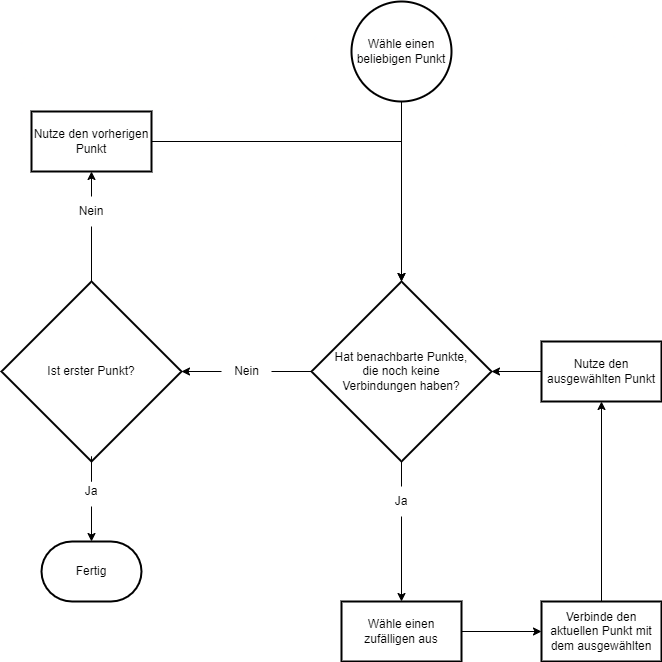
\includegraphics[width=\paperwidth/2]{../assets/img/Randomised-Depth-First-Search}
        \caption{Randomized-Depth-First-Search Ablauf}
        \label{fig:randomized-depth-first-search-flow}
    \end{figure}
Gegeben ist ein Feld der Breite $w$ und Höhe $h$.
Das Feld beinhaltet alle Punkte $p\in\{(x,y)\in\mathbb{N}^2, 0\leq x<w, 0\leq y<h\}$.
Daraus wird zunächst ein beliebiger Startpunkt ausgewählt.
Die benachbarten Punkte werden nach Punkten durchsucht, die noch keine Verbindungen haben.
Der Startpunkt wird zufällig mit einem dieser Punkte verbunden.
Anschließend wird der Verbindungspunkt zum neuen Startpunkt.
Hat der Startpunkt keine benachbarten Punkte ohne Verbindungen, so wird der vorherige Startpunkt überprüft.
Dies wird wiederholt, bis es keinen Punkt mehr gibt, der keine Verbindung hat.
Der Ablauf ist auch in Abbildung~\ref{fig:randomized-depth-first-search-flow} dargestellt.

\subsection{Unsere Implementierung}\label{subsec:unsere-implementierung}
    \begin{figure*}[ht!]
        \lstinputlisting[label={lst:randomised-depth-first-search-code}, caption={Randomized-Depth-First-Search Implementierung}, language=java]{../assets/code/recursive_randomised_depth_first_search.java}
    \end{figure*}
Wir haben uns für den \qq{Randomised-Depth-First-Search} Algorithmus entschieden, da dieser in einer guten Laufzeit von $\Theta(n)$\footnote{Im worst-- sowie bestcase braucht der Algorithmus $n\cdot x+h$ Sekunden, wobei $n$ die Anzahl der Felder ist und $x,h\in\mathbb{R}^+$.} hat und subjektiv schöne Abzweigungen generiert.


Zunächst haben wir eine rekursive Implementierung gewählt.
Dies ist zwar bei der Beschreibung des Algorithmus intuitiver, wollen wir jedoch große Labyrinthe generieren, so kann es zu einer StackOverflowException kommen, weshalb auch noch eine iterative Implementierung geplant ist.

Als Datenmodell dient uns ein ungerichteter Graph.
Graphen sind eine Ansammlung von Knoten, die über Kanten miteinander verbunden sind.
(Siehe Abbildung~\ref{fig:what-is-a-graph})
Knoten haben einen Wert und Kanten setzen diese in Relation.
Ungerichtet heißt dabei, dass die Verbindung in beide Richtungen gilt.

    \begin{figure}[ht!]
        \centering
        \begin{tabular}{l c}
            Liste &
            \begin{minipage}{0.7\textwidth}
                \centering
                \begin{tikzpicture}[node distance={15mm}, main/.style = {draw, circle,outer sep=0pt}]
                    \node[main] (a) {a};
                    \node[main] (b) [right of=a] {b};
                    \node[main] (c) [right of=b] {c};
                    \node[main] (d) [right of=c] {d};
                    \node[main] (e) [right of=d] {e};

                    \draw (a) to (b);
                    \draw (b) to (c);
                    \draw (c) to (d);
                    \draw (d) to (e);

                    \title{Liste}
                \end{tikzpicture}
            \end{minipage}\\
            \vspace{15mm}\\
            Baum &
            \begin{minipage}{0.7\textwidth}
                \centering
                \begin{tikzpicture}[node distance={15mm}, main/.style = {draw, circle,outer sep=0pt}]
                    \node[main] (a) {a};
                    \node[main] (b) [above right of=a] {b};
                    \node[main] (c) [above right of=b] {c};
                    \node[main] (d) [below right of=b] {d};
                    \node[main] (e) [below right of=a] {e};

                    \draw (a) to (b);
                    \draw (b) to (c);
                    \draw (b) to (d);
                    \draw (a) to (e);


                    \title{Baum}
                \end{tikzpicture}
            \end{minipage}\\
            \vspace{15mm}\\
            Graph &
            \begin{minipage}{0.7\textwidth}
                \centering
                \begin{tikzpicture}[node distance={15mm}, main/.style = {draw, circle,outer sep=0pt}]
                    \node[main] (a) {a};
                    \node[main] (b) [right of=a] {b};
                    \node[main] (c) [below of=b] {c};
                    \node[main] (d) [left of=c] {d};
                    \node[main] (e) [right of=c] {e};

                    \draw (a) to (b);
                    \draw (b) to (c);
                    \draw (c) to (d);
                    \draw (d) to (a);
                    \draw (a) to (c);
                    \draw (b) to (d);
                    \draw (c) to (e);

                    \title{Graph}
                \end{tikzpicture}
            \end{minipage}
        \end{tabular}

        \caption{Was ist ein Graph?}
        \label{fig:what-is-a-graph}
    \end{figure}
In unserem Fall ist der Wert die Koordinate als Punkt $p\in\{(x,y)\in\mathbb{N}^2, 0\leq x<w, 0\leq y<h\}$.
Da die Dimensionen bekannt sind, ist die Menge aller Punkte $P$ abzählbar (eine endliche Menge).
Dies gestaltet die Implementierung einfach, da so nur die Kanten gespeichert werden müssen.

Mit diesen Voraussetzungen fangen wir nun in Code~\ref{lst:randomised-depth-first-search-code} mit einem Startpunkt \lstinline{current} an und lassen uns so lange alle anliegenden Knoten ohne Verbindung ausgeben, bis es keine mehr gibt.
Mit einem zufälligen dieser Punkte aus \lstinline{adjacent} wird jetzt fortgefahren.
Auf unserem Graphen verbinden wir die Knoten an den beiden Punkten.
Danach wird die gegebene Methode rekursiv erneut aufgerufen, dieses Mal mit dem ausgewählten Punkt.


    \section{Erstellen eines Spiels in Processing}\label{sec:erstellen-eines-spiels-in-processing}
        Dieser Abschnitt beschreibt den Entwicklungsprozess, welchen wir im Laufe des Projektes durchlaufen haben, um ein komplettes Spiel in Processing zu erstellen.

\subsection{Erste Schritte in Processing}\label{subsec:erste-schritte}
Da unsere Gruppe erst wenig Erfahrung mit Processing hatte, haben wir zunächst mit dem Framework herumgespielt. Erstellt wurden einzelne kurze Programme, welche Funktionen wie dem Darstellen mehrere Quadrate in Processing erklärten.

\subsection{Umsetzung in 2D}\label{subsec:umsetzung-in-2D}
Nachdem wir genug Grundwissen über Processing hatten, haben wir mit der Entwicklung des Spiels in 2D angefangen. Dies hatte den Vorteil, dass wir die Grundmechaniken in einer einfacheren Umgebung umsetzen konnten, bevor wir in 3D übergingen.

Java ist eine objektorientierte Sprache. Deshalb wurde der Aufbau der Dateien auch objektorientiert geplant. Insgesamt wurden drei zusätzliche Klassen, zur Hauptklasse, erstellt. Eine Klasse kümmert sich um die Logik und Darstellung des Labyrinths. Eine Klasse kümmert sich um die Steuerung und Darstellung des Spielcharakters und die letzte Klasse, hilft bei der Berechnung, ob eine Kollision zwischen dem Charakter und dem Labyrinth auftritt. Gesteuert wird dies alles von der Hauptklasse, welche auch die Instanz von Processing besitzt.

Da es am Anfang noch keine funktionierende Schnittstelle zu unserer Backend und den damit verbundenen Generator für Labyrinthe gab, haben wir ein Labyrinth mit komplett zufälliger Verteilung generiert.
Mit diesem simplen Aufbau, konnten wir schon mit der Umsetzung der einzelnen Klassen beginnen. Erst wurde das Labyrinth dargestellt, dann wurde der Spielcharakter hinzugefügt. Nachdem eine einfache Steuerung in alle Richtungen funktionierte, haben wir uns um die Kollision gekümmert, damit man nicht einfach durch die Wände laufen kann.
\newline BILD von random Laby, ganz früh in der Entwicklung \newline

Als nächstes wurde die erste Schnittstelle für generierte Labyrinthe hinzugefügt, ein einfaches Auslesen einer JSON Datei, welche das Labyrinth in einem Grid gespeichert hat. 
Da die meisten Mechaniken schon zuvor umgesetzt wurden, war das Spiel damit in dem ersten komplett spielbaren Stand.

\subsection{Umsetzung in 3D}\label{subsec:umsetzung-in-3D}
Nachdem das Spiel in 2D funktionierte, sind wir auf 3D umgestiegen. Da, wie zuvor schon erwähnt, Java eine objektorientierte Sprache ist, haben wir möglichst viel Code der 2D Klassen vererbt und im Nachhinein angepasst. 
Das Umsetzen in 3D war für uns besonders interessant, da wir bislang noch nichts in 3D gemacht haben. Deshalb haben wir wieder zunächst die Dokumentationen und Tutorials von Processing durchlaufen, um zu verstehen, wie genau Processing 3D umsetzt. Es stellte sich heraus, dass das Erstellen von Körper in 3D vergleichsweise einfach war, nachdem wir vieles von der 2D Umsetzung übernehmen konnten. Jedoch muss man für die Kamera sehr viel selbst berechnen, da einem nur wenig abgenommen wird. Generell war die Kamerasteuerung einer der größten Hürden in der Umsetzung der 3D Ansichten.
Es wurden 2 Ansichten umgesetzt, wobei wir erst uns auf eine Top-Down Ansicht fokussiert haben. Dies lag unter anderem daran, dass die Steuerung des Spielcharakters der der 2D Ansicht ähnelte. Bei einer Top-Down Ansicht, sieht man ähnlich, wie bei einer 2D Ansicht von oben auf das Spielfeld. Teilweise wird dies auch gerne als Vogelperspektive bezeichnet, da die Kamera und damit der Spieler wie ein Vogel von oben schaut. 
\newline BILD 3D TOPDOWN \newline

Als die Top-Down 3D Ansicht unseren Wünschen entsprach, erstellten wir auch schon die ersten Anfänge einer First-Person 3D Ansicht. Mit einer First-Person Ansicht meint man eine Ansicht, welche die Perspektive des Spielers selbst besitzt. Im Falle unseres Labyrinthes bedeuted dies also, dass man selbst im Labyrinth steckt und nicht einfach über die Wände schauen kann. 
\newline BILD 3D First-Person \newline

Da es sicher herausstellte, dass wir dabei noch eine Hand voll mehr Hürden haben werden, fokussierten wir uns erst auf die Verschönerung der allgemeinen 3D-Ansicht. Wie man auf den Bildern erkennen kann, war die Spielwelt sehr einfarbig. Deshalb erkundigten wir uns, wie man Texturen in 3D einfügt. Dabei lernten wir, dass die Standardfunktion für einen einfachen Würfel keine Möglichkeiten für Texturen gaben. Als Lösung haben wir stattdessen eigenen Würfel mithilfe von kombinierten 2D Flächen erstellt. Diese einzelnen Flächen kann man einfach mit einer Textur versehen, die als ganzes die Wände unseres Labyrinthes darstellten.
\newline BILD 3D TopDown MIT TEXTUR \newline

Das Spiel sah nun viel schöner aus. \newline
Kommentare WIP \newline
- 3D First Person klappte\newline
- Optimierung für fast grenzenlose Labys \newline
- ALLE BILDER noch hinzufügen \newline

    \newpage
    \pagenumbering{roman}
    \printbibliography
\end{document}